%!TEX root = ../thesis.tex

% FIGURE: instantaneous luminosity
\begin{figure*}[p]
  \vspace{-6mm}
  \centerline{
    %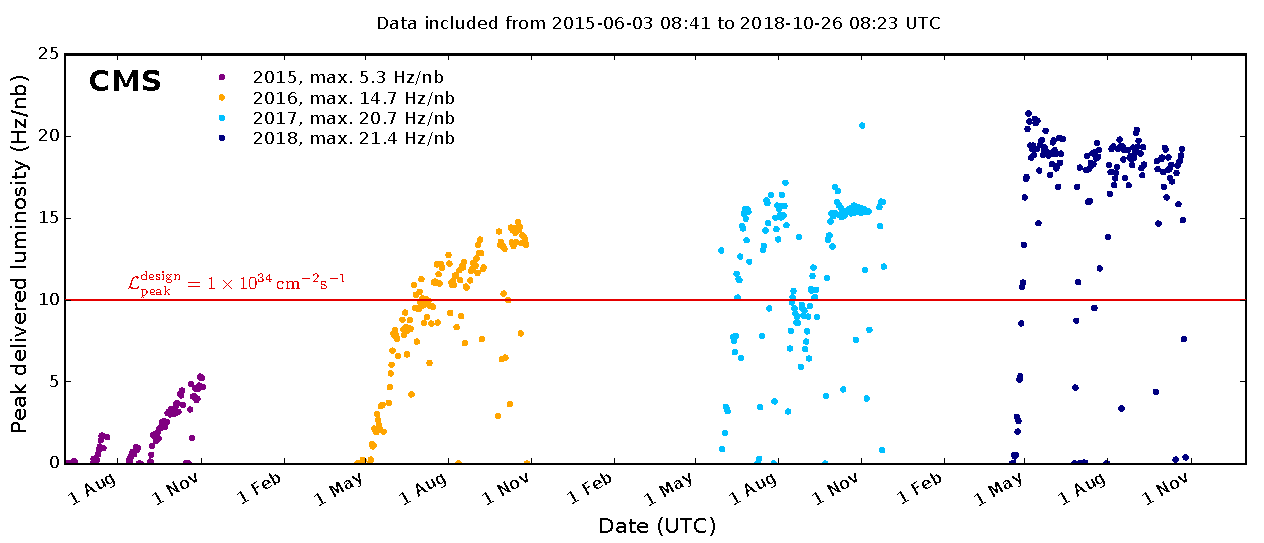
\includegraphics[width=1.04\textwidth,clip,trim={30mm 0mm 16mm 10mm}]{fig/detector/CMS_luminosity_peak_Run2_edit.pdf}
    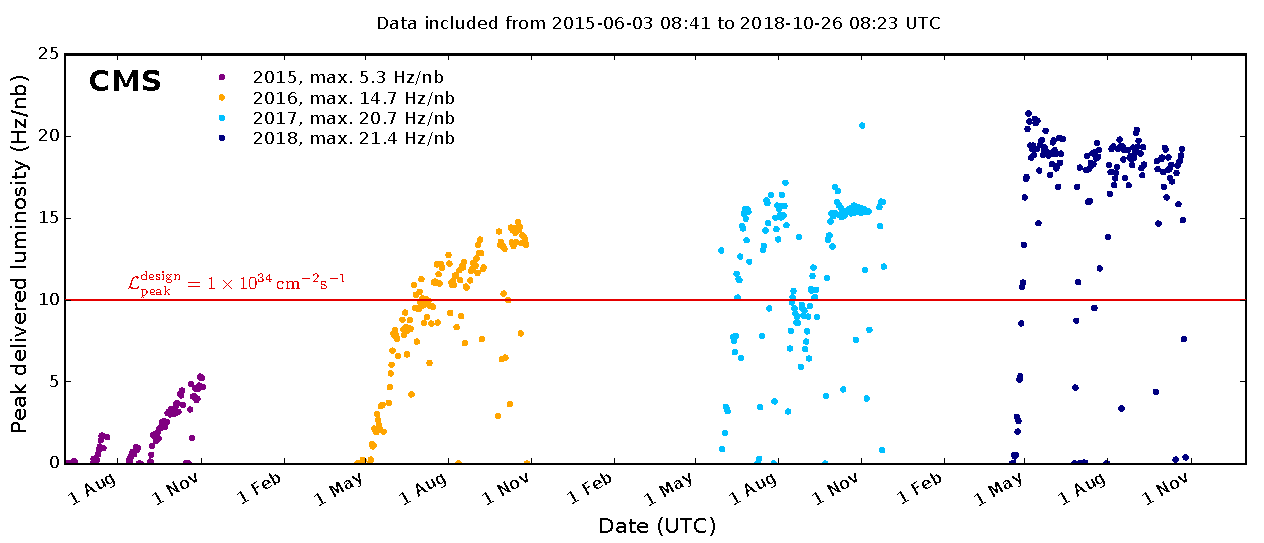
\includegraphics[width=1.04\textwidth]{fig/detector/CMS_luminosity_peak_Run2_edit.pdf}
  }
  \caption{
The instantaneous luminosity \lumi.
The design luminosity is $\lumi^\text{design}_\text{peak}=10^{34}\unit{cm}^{-2}\unit{s}^{-1}$.
Adapted from~\cite{CMS_lumi_TWiki}.
  }\label{fig:CMS_peak_lumi}
  \vspace{-3mm}
\end{figure*}

% FIGURE: integrated luminosity
\begin{figure*}[p]
  \centering
  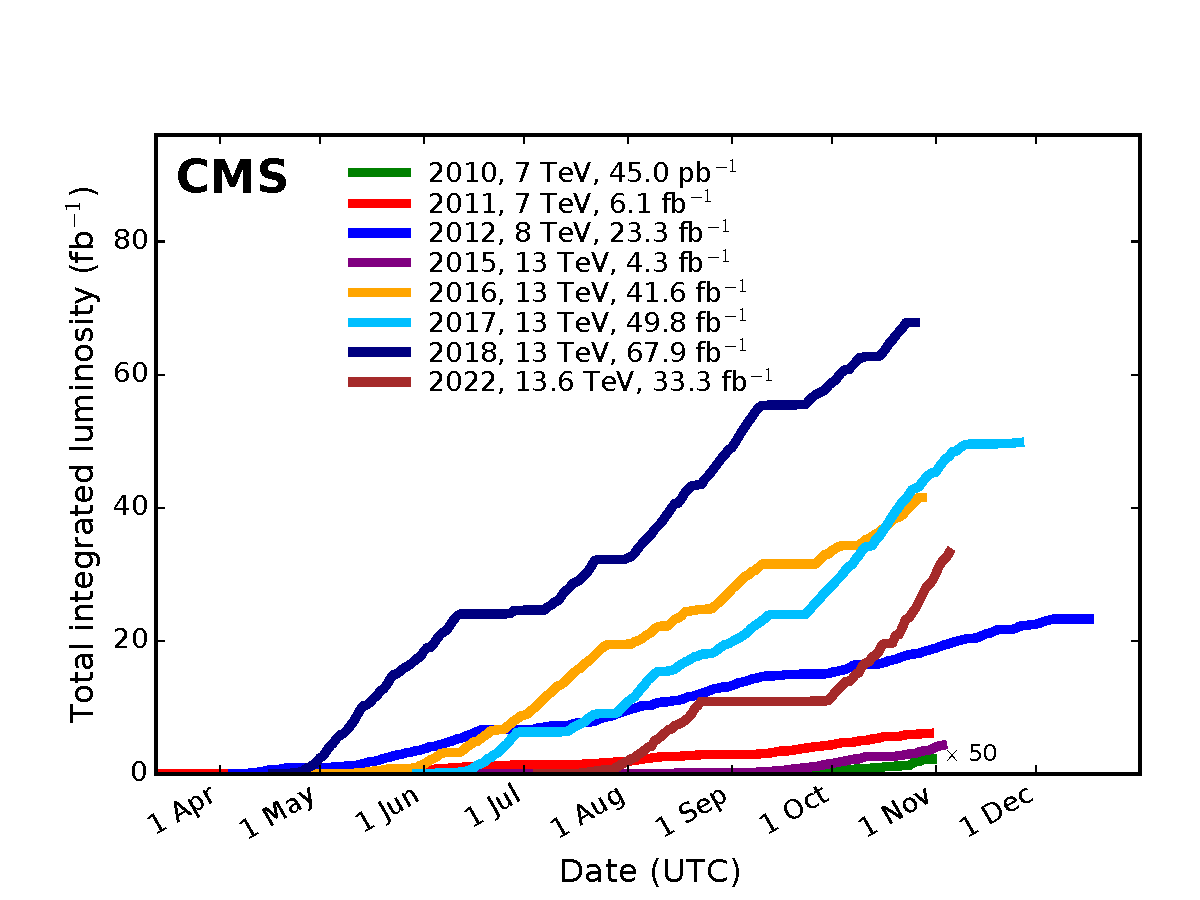
\includegraphics[width=0.57\textwidth,clip,trim={6mm 0mm 6mm 20mm}]{fig/detector/CMS_luminoisty_integrated_Run2.pdf}
  \caption{
Integrated luminosity collected by CMS at $\sqrt{s}=13\TeV$.
Figure taken from~\cite{CMS_lumi_TWiki}.
  }\label{fig:CMS_lumi}
  \vspace{-3mm}
\end{figure*}

% FIGURE: luminosity and pileup
\begin{figure*}[p]
  \centering
  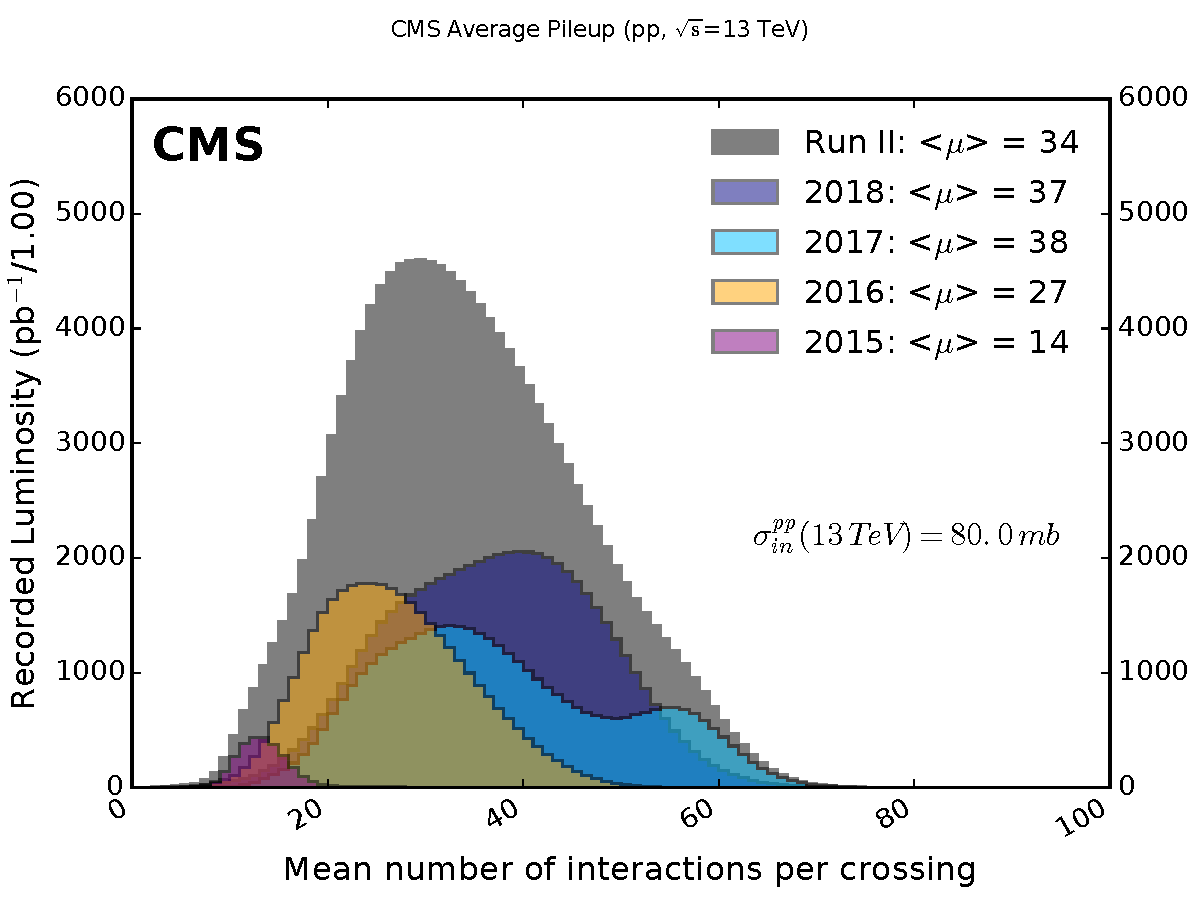
\includegraphics[width=0.58\textwidth,clip,trim={0mm 0mm 0mm 10mm}]{fig/detector/CMS_pileup_Run2.pdf}
  \caption{
Distribution of number of pp interactions, assuming an inelastic cross section of $80\unit{mb}$.
Figure taken from~\cite{CMS_lumi_TWiki}.
  }\label{fig:CMS_pileup}
  \vspace{-4mm}
\end{figure*}
